%!TEX root = Manuscript.tex

\chapter{Proof of feasibility}
\label{chap:TSN}
\minitoc

We showed on this thesis algorithms to compute the lowest latency possible in serveral kind of networks. As we explained, it is necessary that packets are not delayed in the network. Delay causes are various, but the main one if the buffering time. 

This chapter present in Section~\ref{sec:TSNqbv} the IEEE standards for Time Sensitive Networking (TSN) task group, that allows a better network managment based on scheduled packets and on which our model is based.

The platform presented in Section~\ref{sec:platform} goes beyond TSN, by delivering packet at exact expected dates, achieving what we call “Hyper TSN”. In Hyper TSN, the latency is as close as possible with physical limitations.


\section{A Customized Managment of the Network}
\label{sec:TSNqbv}

Our approach of the network is related to the concept of Deterministic Networking. A working group from IETF called DetNet~\cite{finn-detnet-architecture-08} works in collaboration with TSN (Time Sensitive Networking)~\cite{ieee802}, a task group of IEEE, to develop technical solutions for deterministic networking. While DetNet works on Layer 3, TSN devlop solutions for Layer 2. Since our model is based on ethernet we focus on TSN standards.

\subsection{TSN Standards : tools for deterministic networking}
The model we present in Chapter~\ref{chap:model} is based on several assumption. We explain in this chapter how the recent standards developed by TSN task group brings us to such a model. A detailled survey of all TSN standards can be found in~\cite{8458130}. 


The stadard IEEE 802.1Qat SRP~\cite{article} (Stream Rerservation Protocol) provides a central managment framework that allow a centralized entity to collect datas about the flows over the network and to reserve bandwidth for the flows. It has been improved by IEEE 802.1Qcc~\cite{6755436}. Those standards allows us to centralize all required information needed by our algorithm about the network (the routing, the length of the links, the periodicity andthe size of the datagrams) in a centralized entity that we call \textbf{controller}. This controller propose an user interface that allows us to collect all network information in order to compute the best solution with the algorithms of previous chapters. Figure~\ref{fig:networkcontroller} shows a network managed by a controller, communicating via its user interface with users algorithms, and able to send requirement to the nodes. Such an approach is related to Softward Defined Network (SDN)~\cite{li2015software}. We can find in~\cite{7356556} a good example of SDN for TSN.


\begin{figure}
\begin{center}
\scalebox{0.4}{

\begin{tikzpicture}
  \SetGraphUnit{5}
    \tikzset{
  EdgeStyle/.append style = {->} }
   \tikzstyle{VertexStyle}=[shape = circle, draw, minimum size = 30pt]
 

  \node (r1) at (0,0) {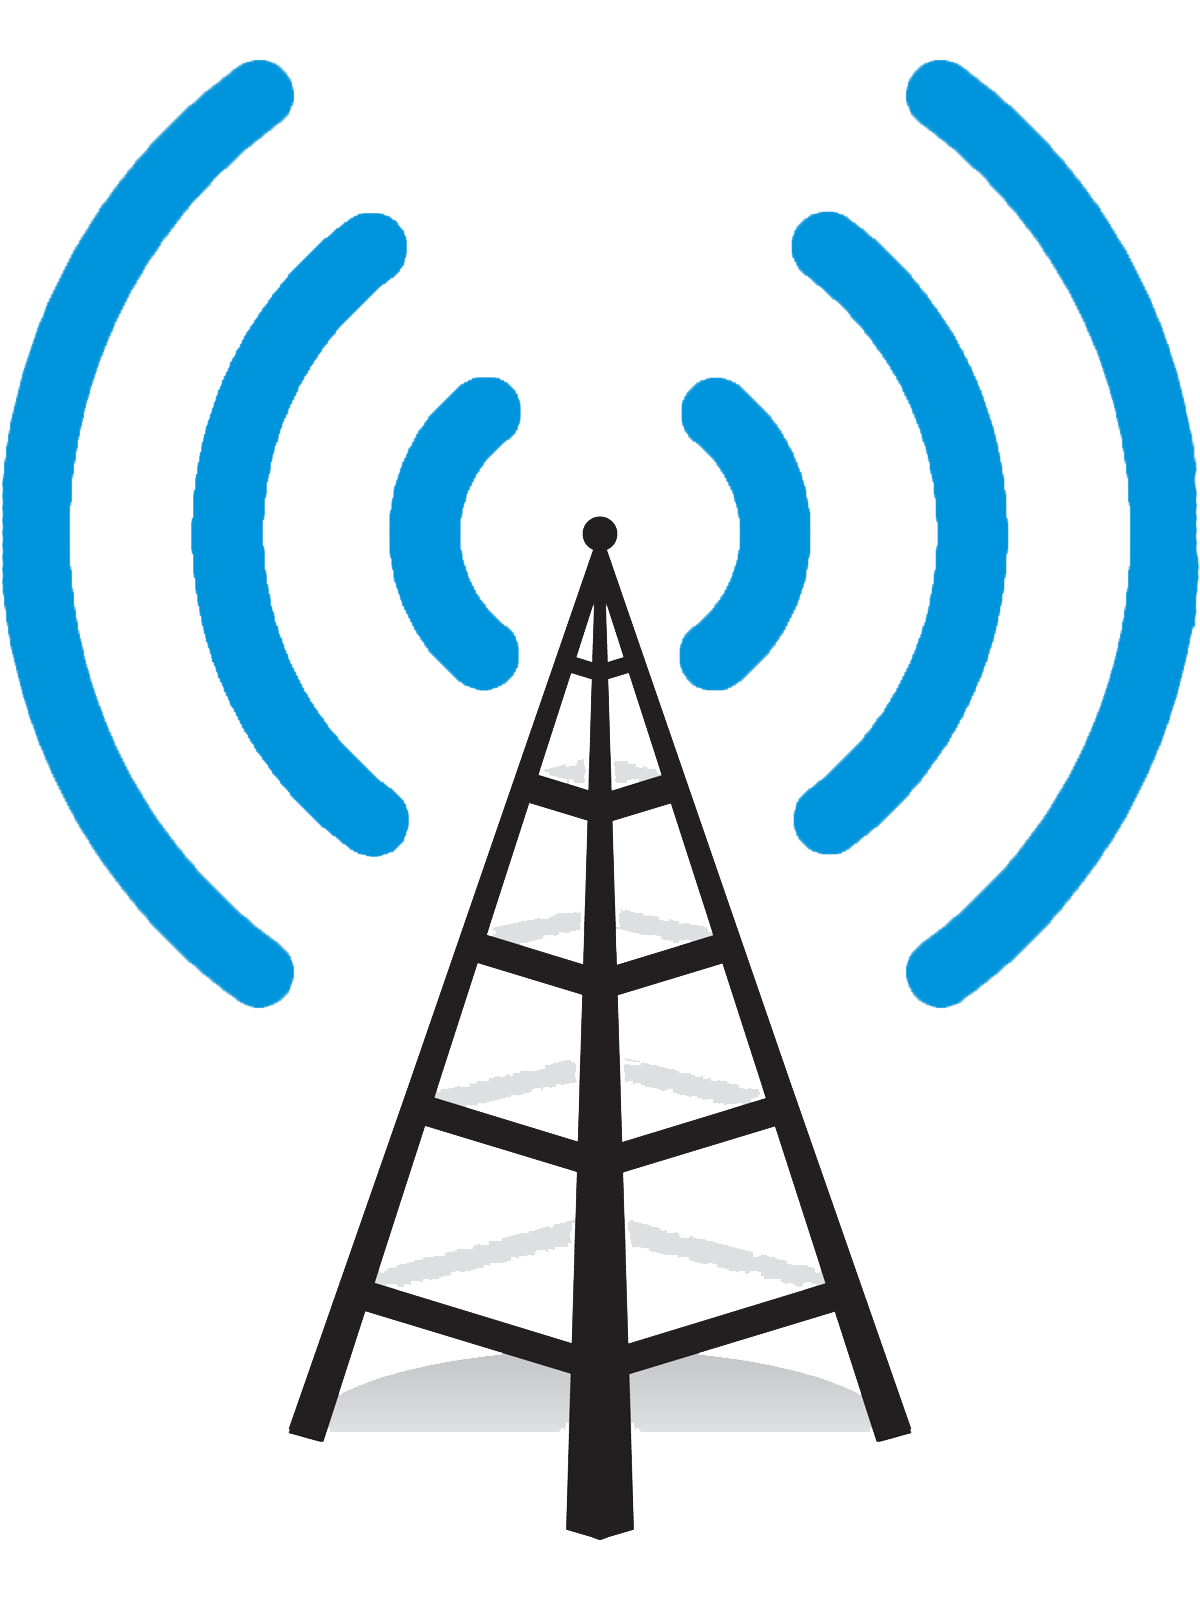
\includegraphics[width = 1cm]{rrh.png}};
   \node[below] at (r1.south) {RRH};
  \node (r2) at (0,4) {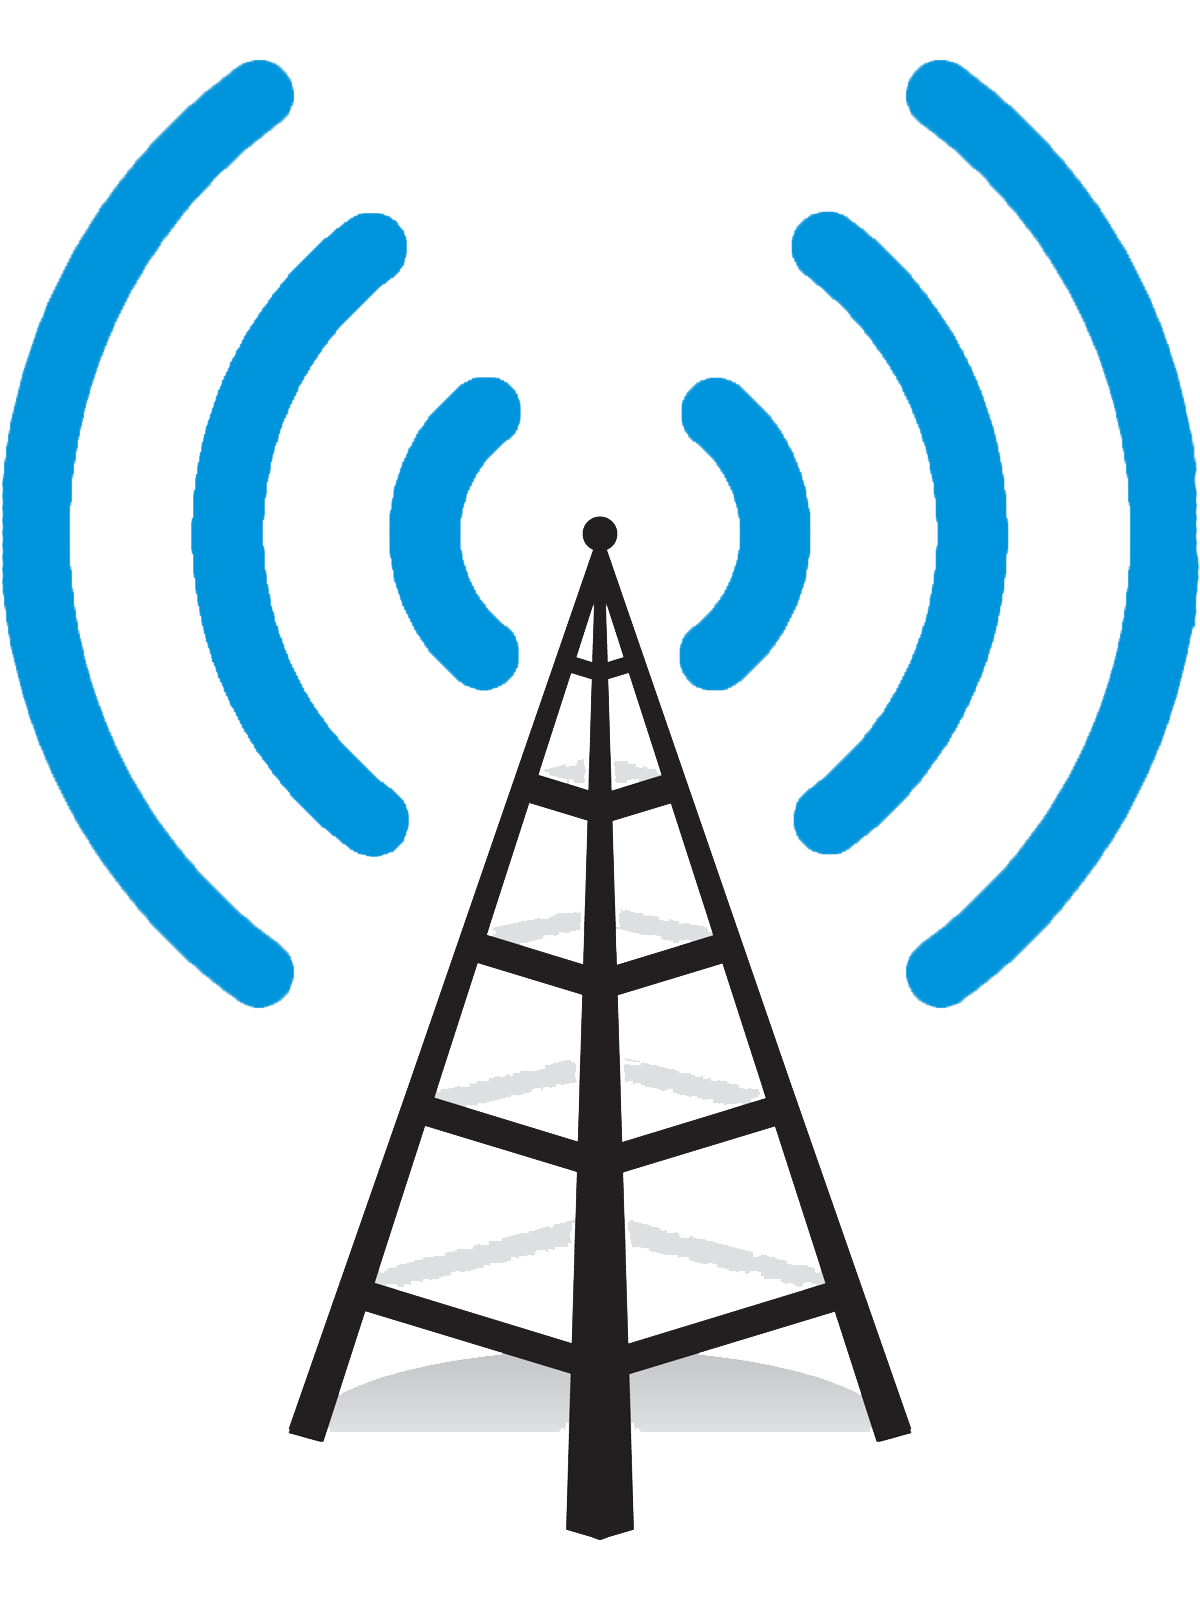
\includegraphics[width = 1cm]{rrh.png}};
   \node[below] at (r2.south) {RRH};
   \node (b1) at (12,0) {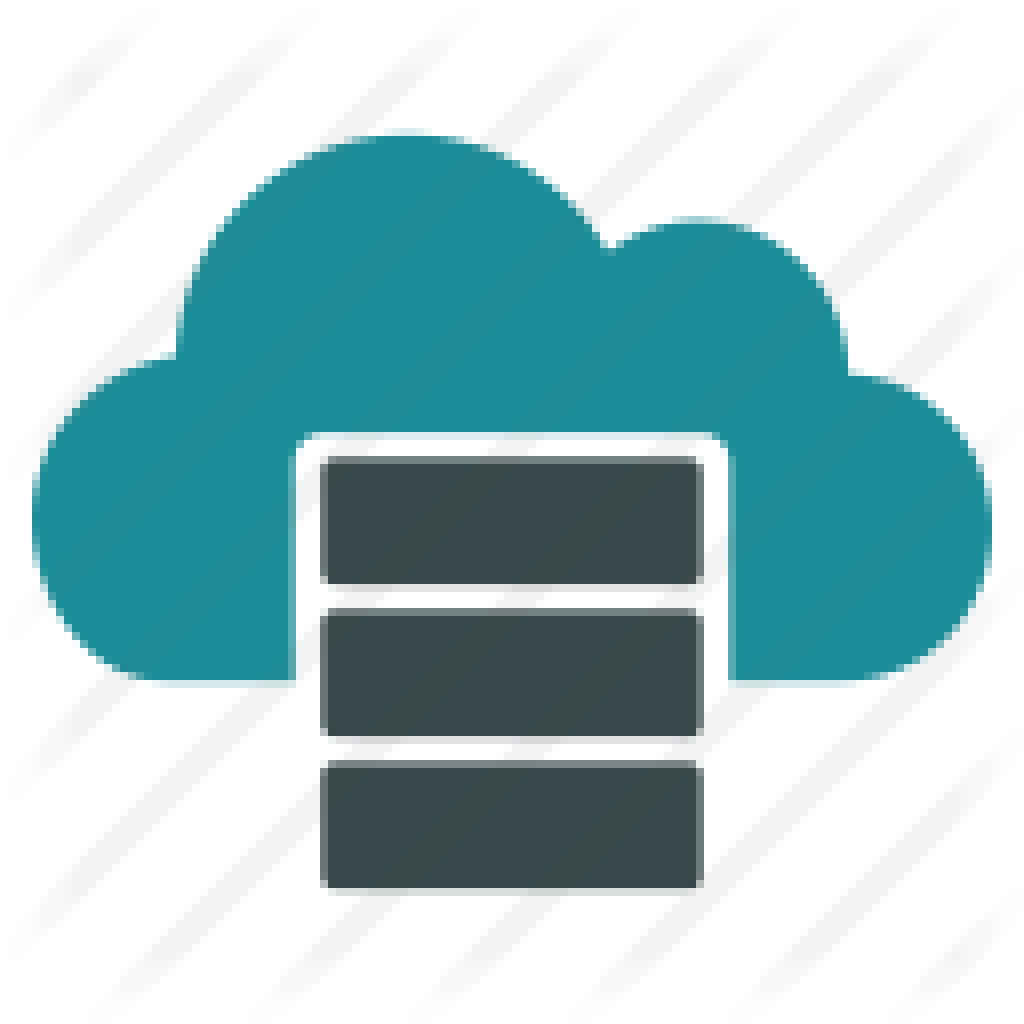
\includegraphics[width = 1cm]{bbu.png}};
   \node[below] at (b1.south) {BBU};
   \node (b2) at (12,4) {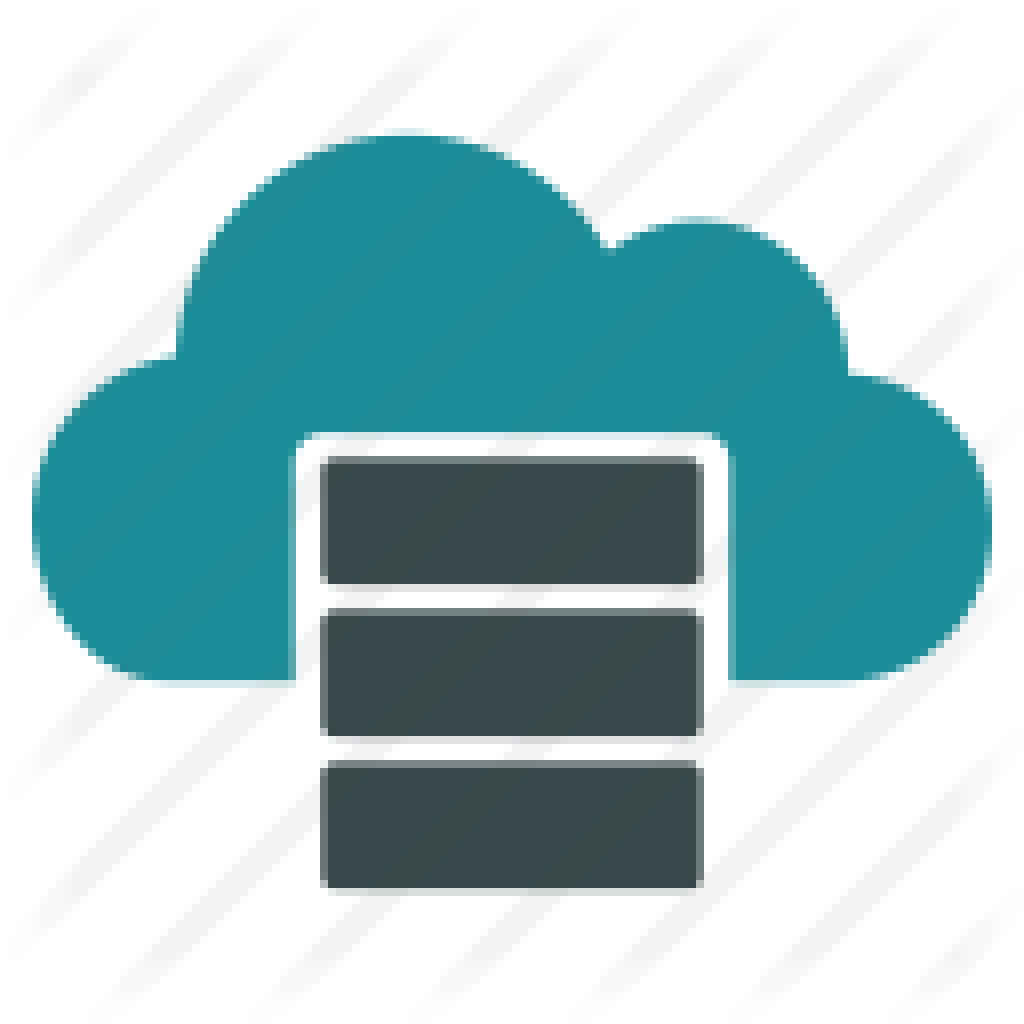
\includegraphics[width = 1cm]{bbu.png}};
	\node[below] at (b2.south) {BBU};
   \node (s1) at (4,2) {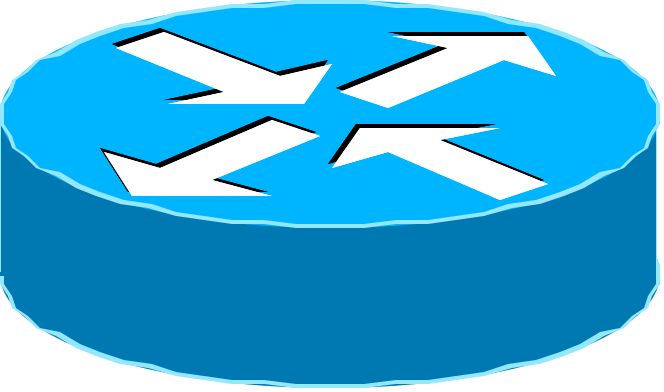
\includegraphics[width = 1cm]{switch.png}};
   \node (s2) at (8,2) {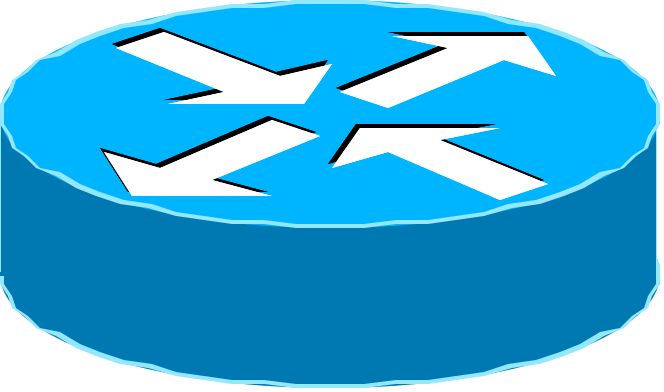
\includegraphics[width = 1cm]{switch.png}};
  
   \node (c) at (6,6) {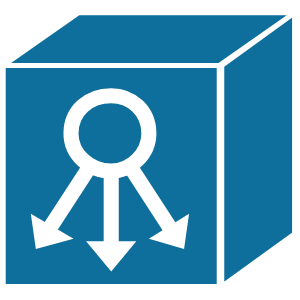
\includegraphics[width = 1cm]{controller.png}};
   	\node[right] at (c.north east) {Controller};

   	\node (rect) at (6,10) [draw,thick,minimum width=2cm,minimum height=1cm] {Algorithms};

\path (r1) edge [<->]  (s1);
\path (r2) edge [<->]  (s1);
\path (s2) edge [<->]  (s1);
\path (s2) edge [<->]  (b1);
\path (s2) edge [<->]  (b2);
\path (s2) edge [<->]  (c);
\path (s1) edge [<->]  (c);
\path (r1) edge [<->]  (c);
\path (r2) edge [<->]  (c);
\path (b1) edge [<->]  (c);
\path (b2) edge [<->]  (c);
\path (rect) edge [<->]  (c);


\end{tikzpicture}
}


 \caption{A TSN network managed by a cotroller, able to collect network informations, compute the GCL and send it to the nodes.}

\label{fig:networkcontroller}
\end{center}
\end{figure}


Once the scheduling of the datagram is computed, switches needs to be able to forward the packet at the right exact date, differentiating the flows, without any additional latency. 

802.1Qbv~\cite{8613095} allows us to manage flows in the nodes by a gate mechanism. The switch schedules on each node the date at which a flow must be sent on each output port. To do so, the switch needs a Gate Control List (GCL). This GCL is computed by our algorithm, and sent to each switch of the network by the controller. It is a list of date, and for every date of the list are specified the output ports (gates) of the switch which are open or close.
Figure~\ref{fig:tsnqbv} found in~\cite{durr2016no} shows the mechanism of a switch using 802.1Qbv technology. Considering a given period ($T_{cycle}$ in the figure), the switch selects at each time ($T_1 , T_2 , \ldots$ the queues that must be open to transmit packets. In figure 6, at time $T_1$, all gates except the one for scheduled traffic are open, at time $T_2$, all gates are closed and at time $T_3$ only the gate for scheduled traffic is open.
  \begin{figure}
      \begin{center}
      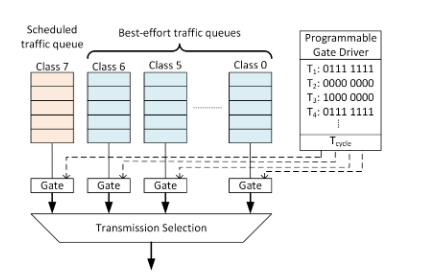
\includegraphics[width=0.8\textwidth]{Chapitre1/tsnqbv.png}
      \end{center}
      \caption{IEEE 802.1Qbv mechanism}\label{fig:tsnqbv}
      \end{figure}
      
With such a mechanism, it is possible let the C-RAN flows cross the nodes at the exact time they arrive. To do so, it is necessary to compute the CGL upstream. Furthermore, it is essential to schedule the different C-RAN flows so that two flows never use the same resource at the same time.
   
We consider that the components of the network are completely synchronized. Such an hypothesis seems unrealistic, but standards likes IEEE 802.1AS~\cite{5741898}, or IEEE 1588~\cite{4579760} propose good solutions for clock synchronization. This issue is fully covered by Hyper-TSN switch of the next section \todo{J'en sais rien en fait?}.

All those standards allows us a precise managment of the network. Nevertheless, there is still some additional delays due to several sources : \todo{demander a brice}.


\section{An experimental prototype}
\label{sec:platform}
- On sait faire des noeuds qui respectent l'organisation

- On sait comment ne pas buffuriser du tout les messages: PALL PAZL

-Voir comment gérer le problème de Dsynch

-parler des reseaux sans aucun buffers intermediaires evoqués dans les chapitres PAZL et PALL
\subsection{Hyper-TSN switch}
In store-and-forward concept~\cite{tindell1992store}, packets are stored at reception of a node before to be forwarded. However, solution like cut-through~\cite{kermani1979virtual} allow to reduce storage size and corresponding delay to the header size only. But this is effective if the egress port is available to forward the packet at the same time only. If not, the packet is buffered until the port get free. This situation needs to be avoided.

An Hyper-TSN switch has been developped. It is composed of a deterministic scheduler, two 10 Gbps ethernet ingress and two 10 Gbps ethernet egress ports. The deterministic scheduler is configured with a timing table. This table is similar to a 802,1 Qbv Gate Control List (GCL). It defines the periodicity of the scheduling and, for each port, the planed date of arrival of the datagrams. At each of these dates the deterministic scheduler sets the switch to transmit data incoming on a specified ingress port.

To perform experiments a generator of deterministic flows has been developed on a Xilinx FPGA board,Zynq-7000 SoC zc706. This generator offsets the dates it sends the frames according to the controls received from the monitoring circuitry.

To perform the experiment the generator is configured to send frames on both egress ports according to the period defined in the timing table. The size of the frames is set to fully load the ethernet links (ie $100\%$ load).

When starting, the monitoring circuitry detects that frames do not arrive at the planed date and sends control commands to the generator. These first frames are lost. Once the generator has rightly offset the dates it sends the frames, nor more offset has been performed during the running 2 hours experiment.

Then $100\%$ of the frames are correctly switched without being corrupted or lost. The switching of each frame from the ingress port to the planed egress port is performed introducing only one clock cycle delay (here 3,87 ns).
